\documentclass{beamer}

\usepackage{multicol}
%\usepackage[dvipsnames]{xcolor}
\usepackage{graphicx}
\usepackage{pifont}
\usepackage{multirow}
\usepackage{ragged2e}
\usepackage{changepage}
\usepackage{adjustbox}

\usepackage{wrapfig}

\usepackage[margin=1in, top=1.25in, headheight=2\baselineskip, headsep=\baselineskip]{geometry}


% Grafici
\usepackage{graphicx, booktabs, wrapfig, pdfpages}
\usepackage{pgfplots}
\usepackage[framemethod=tikz]{mdframed}
\usepackage[outline]{contour}
\usepackage[ labelfont=bf, labelsep=period, margin=0.5in]{caption}\usepackage{pdfpages}
\usepackage[labelfont=bf, labelsep=period, margin=0.5in]{caption}

\usepackage{upgreek} %per scrivere mu non corsivo (\upmu)

% Use Unipd as theme, with options:
% - pageofpages: define the separation symbol of the footer page of pages (e.g.: of, di, /, default: of)
% - logo: position another logo near the Unipd logo in the title page (e.g. department logo), passing the second logo path as option 
% Use the environment lastframe to add the endframe text
\usetheme[pageofpages=of]{Unipd}

\title{Proprietà dei candidati Muoni del Trigger L1 di CMS}
%\subtitle{Demonstrating how to use the Unipd theme}
\author[La Rovere Francesco]{La Rovere Francesco}

\date{9 Dicembre, 2024}

\AtBeginSubsection[]
{
  \begin{frame}
  \large

    \frametitle{Indice analitico}
    \tableofcontents[currentsection, subsectionstyle=show/shaded]
  \end{frame}
}

\begin{document}
\footnotesize

% Make the title page
\frame{\titlepage}

\section{Introduzione}

\begin{frame}{LHC e CMS}

Situato a Ginevra, Svizzera, il Large Hadron Collider è il più grande acceleratore di particelle mai costruito. 

\begin{columns}
    \begin{column}{0.55\textwidth}
        \begin{itemize}            
            \item Collisione di protoni a $\sqrt{s} \approx 14$ TeV
            \item Collisioni ogni 25ns (BX) $\rightarrow$ 40 milioni di iterazioni al secondo
        \end{itemize}

        CMS esperimento multifunzionale
        \begin{itemize}
            \item Raccogliere e studiare informazioni sui prodotti di collisione
            \item Studiare fenomeni esotici
            \item Selezione eventi $\rightarrow$ sistema di Trigger a due livelli, L1T e HLT
        \end{itemize}
    \end{column}
    \begin{column}{0.4\textwidth}  
    \centering
       \scalebox{0.1}{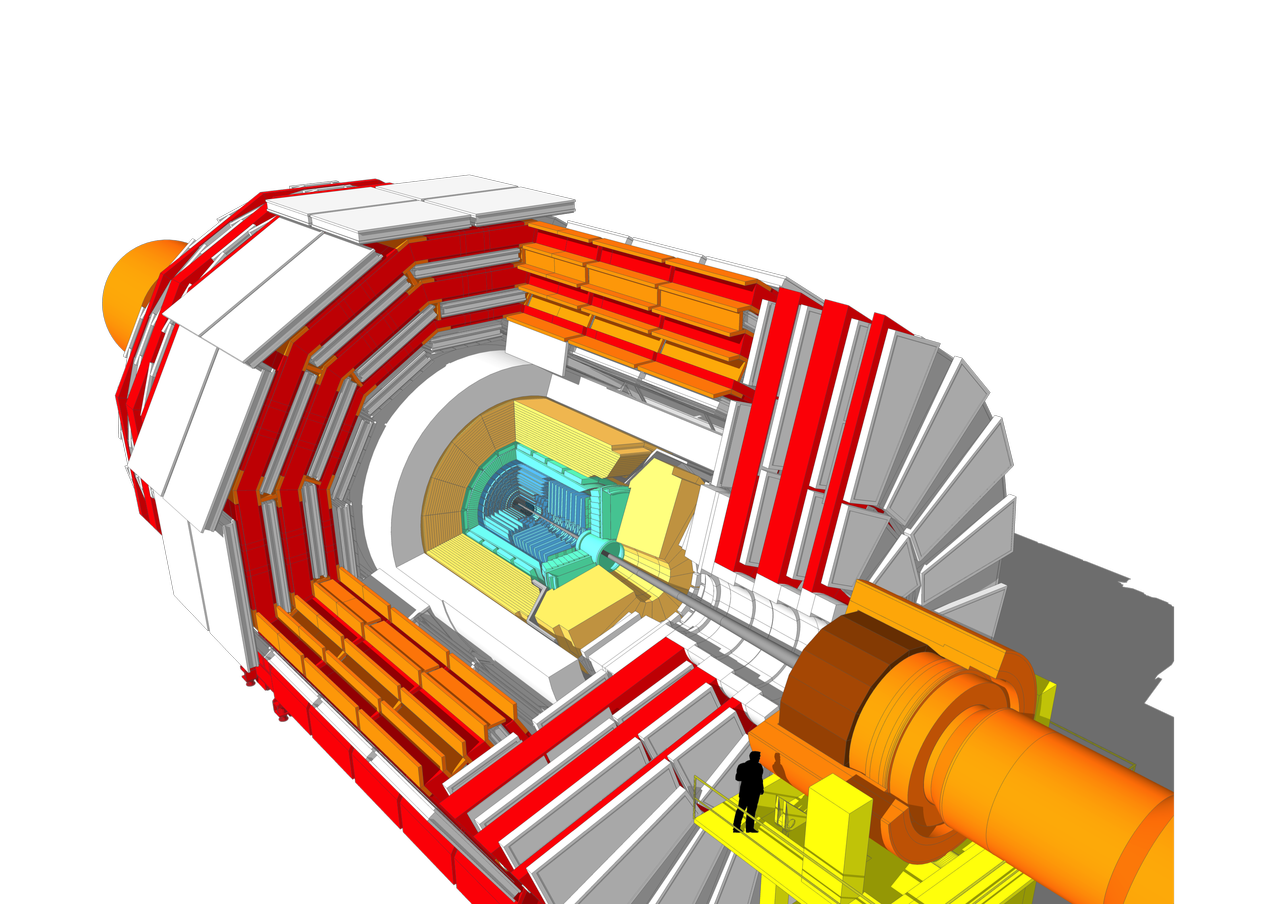
\includegraphics{Immagini/CMS.png}} 
       \vskip 0.5cm % Aggiunge uno spazio verticale di 0.5cm
       \scalebox{0.33}{\includegraphics{Immagini/ropac5106f6_hr.jpg}}
    \end{column}
\end{columns}

\end{frame}



\begin{frame}{Data Scouting}

Il Trigger scarta la quasi totalità degli eventi (99.75\%), 40MHz $\rightarrow$ 1kHz:


\begin{columns}
    \begin{column}{0.50\textwidth}
        \begin{itemize}            
            \item Introduzione di un bias 
            \item Occultamento di segnali di Nuova Fisica
        \end{itemize}
        \vspace{0.2 cm}
        Sistema di Data Scouting nel L1T introdotto con la Run 3:
        \begin{itemize}
            \item Analisi degli eventi all'inizio della catena di Trigger
            \item Minore risoluzione, maggiore statistica
            \item Nessun bias introdotto

        \end{itemize}
    \end{column}
    \begin{column}{0.5\textwidth}  
    \centering
       \scalebox{0.28}{\includegraphics{Immagini/scouting.png}}  
    \end{column}
\end{columns}
    
\end{frame}




\section{Proprietà dei candidati Muoni}

\begin{frame}{Trigger Superprimitives}

\begin{columns}

    \begin{column}{0.5\textwidth}
    Zona centrale di CMS (barrel):
    \begin{itemize}
        \item Eventi di background minimi
        \item Sono impiegati DT e RPC
    \end{itemize}
    \vspace{0.5 cm}
    Le schede TwinMux (concentratori):
    \begin{itemize}
        \item Generano superprimitives combinando segnali dei DT e RPC
        \item Assegnano a ciascuna superprimitives parametri spaziali e qualitativi.
    \end{itemize}

    \end{column}
    \begin{column}{0.5\textwidth}
        \centering
        \scalebox{0.18}{\includegraphics{Immagini/TriggerSystemTwinMux.png}} 
    \end{column}
\end{columns}
    
\end{frame}


\begin{frame}{BMTF Muons}

\begin{columns}

    \begin{column}{0.5\textwidth}
    Sistema di Tracking BMTF:
    \begin{itemize}
        \item Ricostruzione delle tracce dei muoni dalle stubs implementata in hardware 
        \item Algoritmo Kalman filter
    \end{itemize}
    \vspace{0.3cm}
    Estraendo informazioni delle schede TwinMux:
    \begin{itemize}
        \item Emulazione software del sistema di Tracking $\rightarrow$ maggiore risoluzione
    \end{itemize}
    

    \end{column}
    \begin{column}{0.5\textwidth}
        \centering
        \scalebox{0.18}{\includegraphics{Immagini/TriggerSystemBMTF.png}} 
    \end{column}
\end{columns}

\end{frame}


\begin{frame}{GMT Muons}

\begin{columns}

    \begin{column}{0.5\textwidth}
    
    Il GMT ha il compito di selezionare i migliori 108 candidati muoni dei 3 sistemi di tracking in base a:
    \begin{itemize}
        \item Qualità
        \item Momento trasverso $p_T$
        \item Regione di provenienza
    \end{itemize}
    \vspace{0.3cm}

    È interessante verificare il confronto tra muoni del GMT, raccolti dal sistema di DS, e candidati muoni emulati dal software del BMTF.

    

    \end{column}
    \begin{column}{0.5\textwidth}
        \centering
        \scalebox{0.18}{\includegraphics{Immagini/TriggerSystemGMT.png}} 
    \end{column}
\end{columns}

\end{frame}

\subsection{Confronto Muoni del BMTF con Muoni del GMT}


\begin{frame}{Confronto BMTF e GMT Muons}

Il confronto avviene ricercando le coppie di muoni più vicine spazialmente:
\begin{itemize}
    \item Distanza definita da $\Delta R = \sqrt{(\Delta \phi)^2 + (\Delta \eta)^2} < 0.4$

\end{itemize}

\begin{columns}

    \begin{column}{0.5\textwidth}
    In un determinato BX il confronto avviene in due modi
        \begin{itemize}
            \item Fissare un muone del BMTF e verificare la compatibilità con i muoni del GMT (primo metodo)
            \item Fissare un muone del GMT e verificare la compatibilità con i muoni del BMTF (secondo metodo)
        \end{itemize}
    \end{column}
    \begin{column}{0.5\textwidth}
        \centering
        \vspace{0.5 cm}
        \scalebox{0.21}{\includegraphics{Immagini/Confronto/DeltaR.pdf}} 
    \end{column}
\end{columns}

\vspace{0.5 cm}
Per il primo metodo la percentuale di eventi con match è 94.42\% mentre per il secondo è 99.72\%

\end{frame}



\begin{frame}{Studio della Matching Efficiency}
\begin{columns}

    \begin{column}{0.55\textwidth}

    Matching Efficiency in funzione del momento trasverso $p_T$:
    \begin{itemize}
        \item Rapporto tra i muoni con match e muoni totali
    \end{itemize}

    \vspace{0.3cm}

    Primo metodo:
    \begin{itemize}
        \item Decrescita a bassi $p_T$
        \item Crescita a $p_T$ maggiori
    \end{itemize}

    Secondo metodo:
    \begin{itemize}
        \item Maggiore matching efficiency a bassi $p_T$
        \item Leggera decrescita a $p_T$ maggiori
    \end{itemize}
        
    \end{column}
    \begin{column}{0.5\textwidth}
        \centering
        \vspace{0.5 cm}
        \scalebox{0.21}{\includegraphics{Immagini/Confronto/PtMatchingEfficiency.pdf}} 
    \end{column}
\end{columns}

\vspace{0.5 cm}

\end{frame}


\section{Nuova Fisica a CMS}
\subsection{Ricerca Heavy Stable Charged Particles}

\begin{frame}{HSCPs a CMS}
    Tecnica di Data Scouting $\rightarrow$ acquisizione dati unbiased a 40MHz:
    \begin{itemize}
        \item Ricerca di particelle non predette dal Modello Standard
    \end{itemize}

    \vspace{0.3 cm}
    
    Heavy Stable Charged Particles sono particelle massive Long Lived. Principali firme sperimentali:
    \begin{itemize}
        \item \textbf{Velocità ridotta $\beta \ll 1$}
        \item Elevato tempo di volo
        \item Anormale perdita di energia per unità di lunghezza $\langle \frac{dE}{dx}\rangle$
    \end{itemize}

    \vspace{0.3 cm}

    Si cercano segnali di particelle (stubs) che impiegano più di 1BX per attraversare CMS, ovvero:
    \begin{itemize}
        \item Stubs nel BX+1 nella stazione sucessiva rispetto alla stubs nel BX
        \item Stubs bel BX+1 spazialmente vicine rispetto alla stubs nel BX
    \end{itemize}
\end{frame}



\subsection{Studio delle Stubs}
\begin{frame}{Matched Stubs}

Distribuzione delle stubs totali compatibili tra BX e BX+1. Il rate di stubs con match corrisponde a 2.2kHz. 

\vspace{0.6cm}

\begin{columns}

    \begin{column}{0.5\textwidth}
        \scalebox{0.21}{\includegraphics{Immagini/HSCP/MatchedStubs.pdf}} 
    \end{column}
    \begin{column}{0.5\textwidth}
        \scalebox{0.215}{\includegraphics{Immagini/HSCP/MatchedStubsCombination.pdf}} 
    \end{column}
\end{columns}

\vspace{0.5 cm}
    
\end{frame}


\subsection{Studio dei candidati Muoni}

\begin{frame}{Matched BMTF muons}

Studio delle coppie candidati muoni del BMTF in BX adiacenti generati da quattro stubs compatibili (due ognuno):

\begin{columns}

    \begin{column}{0.55\textwidth}
    \begin{itemize}
        \item Rappresentanti probabilmente lo stesso evento
        \item Percepiti dal Trigger come due particelle distinte
    \end{itemize}

    Eventi molto rari, rate $\approx$ 1.4Hz.

    \begin{itemize}
        \item Verificare se sono eventi generati dalla collisione di protoni
        \item Verificare le distribuzioni spaziali e di momento delle differenze delle coppie di muoni
    \end{itemize}
        
    \end{column}
    \begin{column}{0.5\textwidth}
        \scalebox{0.205}{\includegraphics{Immagini/HSCP/BXDiff.pdf}} 
    \end{column}
\end{columns}
    
\end{frame}


\begin{frame}{Matched BMTF muons}

Distribuzione dei momenti relativi $\frac{p_T^{BX} - p_T^{BX+1}}{p_T^{BX}}$ e spaziale $\phi^{BX} - \phi^{BX+1}$ delle coppie di muoni del BMTF in BX adiacenti

\vspace{0.8cm}

\begin{columns}

    \begin{column}{0.5\textwidth}
        \scalebox{0.21}{\includegraphics{Immagini/HSCP/DeltaPt.pdf}}  
    \end{column}
    \begin{column}{0.5\textwidth}
        \scalebox{0.21}{\includegraphics{Immagini/HSCP/DeltaPhi.pdf}} 
        
    \end{column}
\end{columns}
    
\end{frame}


\begin{frame}{Conclusioni}

Studio preliminare $\rightarrow$ informazioni non complete. 
\begin{itemize}
    \item Dataset relativamente piccolo, 5.22 minuti di presa dati
\end{itemize}

\vspace{0.5cm}
Non è stata presa in considerazione:
\begin{itemize}
    \item Velocità delle particelle
    \item Perdita di energia per unità di lunghezza delle particelle
\end{itemize}



\end{frame}

\begin{frame}{Backup}
   Distribuzione delle stubs nei 3564 bunch crossing.

    \vspace{0.5cm}
\begin{columns}

    \begin{column}{0.5\textwidth}
        \scalebox{0.21}{\includegraphics{Immagini/StubsBXnumber.pdf}}  
    \end{column}
    \begin{column}{0.5\textwidth}
        \scalebox{0.21}{\includegraphics{Immagini/StubsBXnumberZoom.pdf}} 
        
    \end{column}
\end{columns}
\end{frame}


\begin{frame}{Backup}
   Distribuzione delle stubs nel corpo di CMS

    \vspace{0.5cm}
\begin{columns}

    \begin{column}{0.5\textwidth}
        \scalebox{0.18}{\includegraphics{Immagini/Stubs/StubsStationWheel.pdf}}  
    \end{column}
    \begin{column}{0.5\textwidth}
        \scalebox{0.18}{\includegraphics{Immagini/Stubs/StubsSectorWheel.pdf}} 
        
    \end{column}
\end{columns}
\end{frame}



\begin{frame}{Backup}
    Distribuzione delle posizioni spaziali nel piano $\eta$ e $\phi$ dei muoni emulati del BMTF e distribuzione del momento vetrex-contrained $p_T$ e unconstrained $p_T^u$.

    \vspace{0.5cm}
\begin{columns}

    \begin{column}{0.5\textwidth}
        \scalebox{0.21}{\includegraphics{Immagini/BMTF/BMTFPhiEta.pdf}}  
    \end{column}
    \begin{column}{0.5\textwidth}
        \scalebox{0.21}{\includegraphics{Immagini/BMTF/BMTF_PtPtu.pdf}} 
        
    \end{column}
\end{columns}
\end{frame}



\begin{frame}{Backup}
    Rappresentazione delle variabili $\phi$ ed $\eta$ di CMS.

    \vspace{0.5cm}
\begin{columns}

    \begin{column}{0.4\textwidth}
        \scalebox{0.35}{\includegraphics{Immagini/dimuon2views_cms.png}}  
    \end{column}
    \begin{column}{0.65\textwidth}
        \scalebox{0.24}{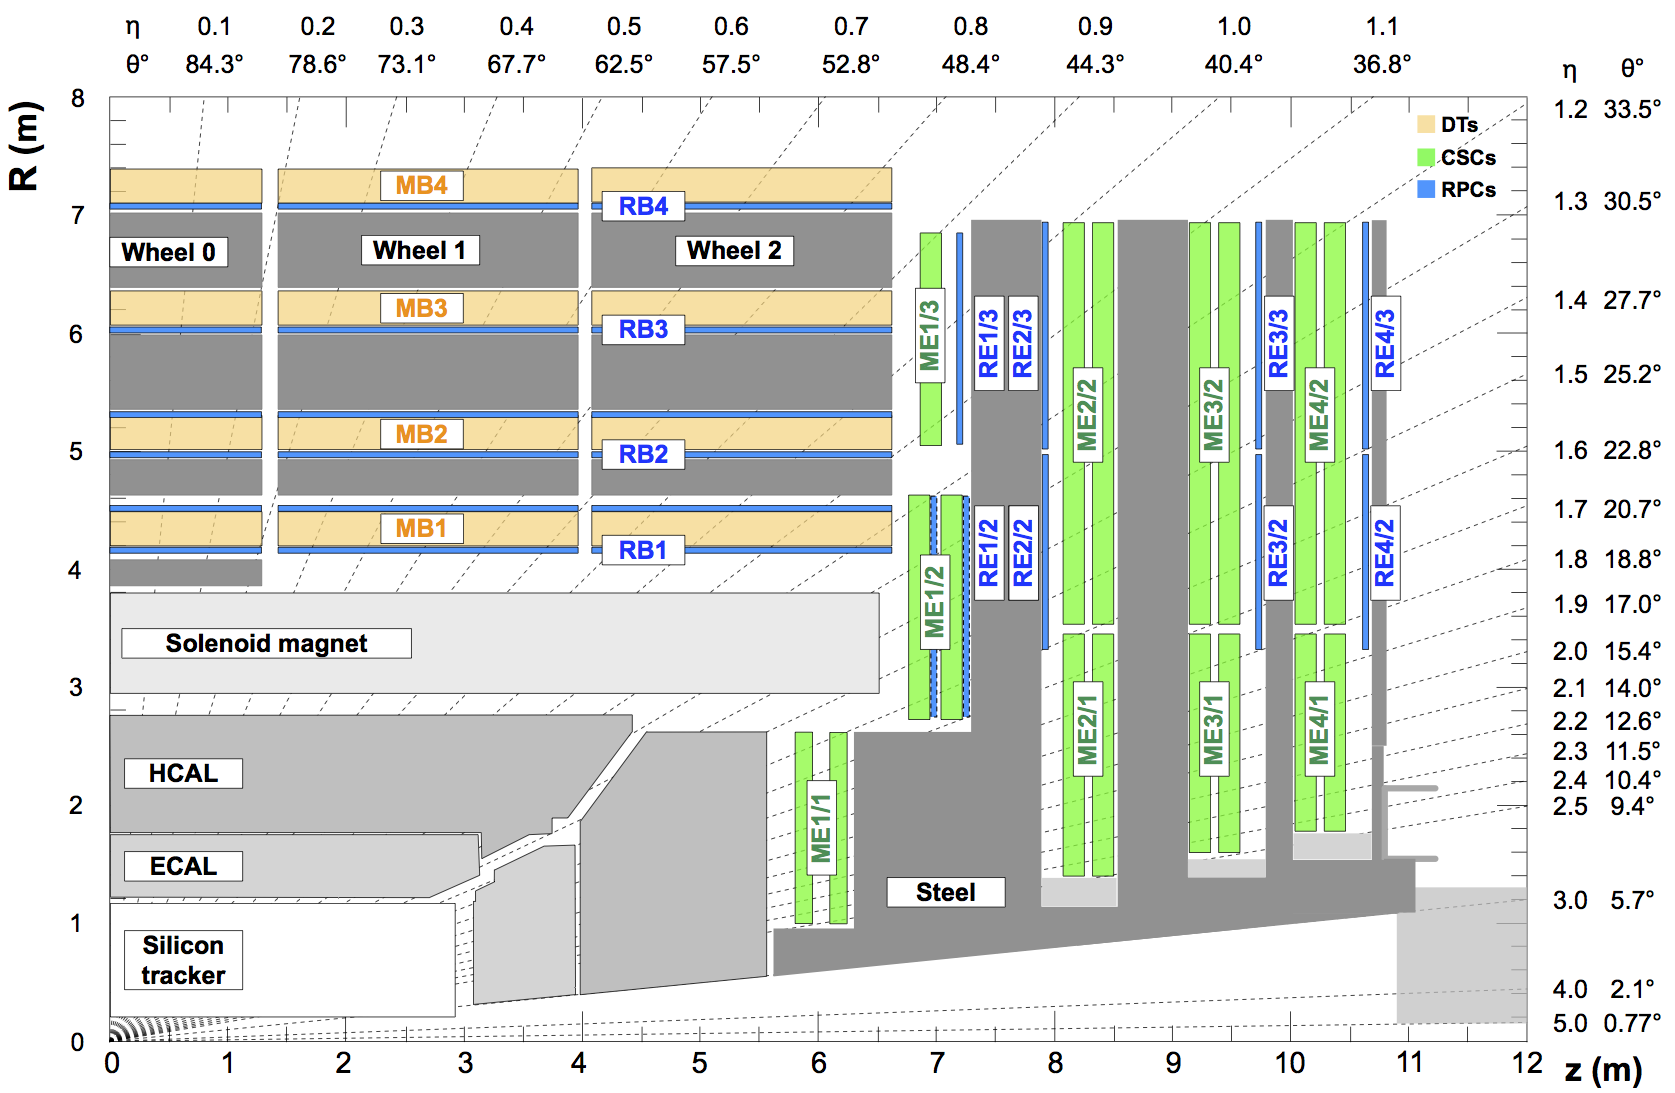
\includegraphics{Immagini/CMSEtaView.png}} 
        
    \end{column}
\end{columns}
\end{frame}





    
    
\end{document}